\chapter{Introduction}
\label{introduction}

\section{Context}
  With the increased availability of smartphones \cite{Statista:2021}, digital cameras \cite{ImarcGroup} and Internet access \cite{Wikipedia} \cite{Globaltt}. Coupled with the increased interest in home food cultivation \cite{Google} and the large number of people reliant on food grown in smallholdings \cite{JLIFADSmallHolders}. The ability to identify defects with crops using technology has potential to be impactful to many people.
\section{Literature Review}
  Firstly, existing research regarding image classification of plants and plant diseases will be
  explored. Secondly, more generalized image classification tasks will be examined and lastly some popular CNN architectures will will be compared.
  \subsection{Disease Detection Usage Of CNNs}
  \par
  In 2009 a study was conducted using deep learning to identify three different disease classes on rice plants. The results showed over 70\% classification accuracy on 50 sample images. The method employed used segmentation, followed by image feature extraction using three different algorithms to extract color, shape and texture information from the image. The feature data was input to a classification algorithm whereby the output would be one of the three disease types or no disease present. \cite{Anthonys2009}
  \par
  In 2015 another experiment (using similar aproach to\cite{Anthonys2009}. Involved using image segmentation
  using using K means clustering and other image processing techniques, to find features in the image and create a one dimensional binary feature vector, to be processed by an ANN. \cite{Khirade2015} The accuracy of detecting powdery mildew, yellow rust and aphids on wheat were 86.5\%, 85.2\%, 91.6\% and 93.5\% respectively.
  This non CNN teqnique has subsequently been rendered redundant as this method requires a greater number of
  computational processes and acheives results that have been surpassed by CNN's. However, the image segmentation teqnique (with the purpose of isolating the leaf from the background) Is also sometimes used in CNN aproaches.
  \par
  A year later and there have been great successes in identifying crop disease with CNN's. In 2016 a paper was published running experiments on a 38 class crop disease dataset over 14 crop species and 26 diseases (or absense thereof). Resulting in 99.35\% accuracy on a held-out test set (using GoogLeNet). \cite{Mohanty2016}. This study utilized two established CNN architectures, namely AlexNet \cite{Krizhevsky} \& GoogLeNet. \cite{Szegedy_2015_CVPR} With GoogLeNet achieving a higher F1 score in almost all cases.
  This study also highlighted the effectiveness of using colour images when training the models. In all experiemnts, the color or segmented image models performed better as appose to grey scale images. A suprising aspect of the results is the fact that the segmented image models almost always permed worse than the colour image models, with the best performing model being trained on colour, non-segmented images. This may be due to some bias being present in backgrounds of the dataset images. Or it may be more effective to not perform segmentation on the images prior to training.
  \par
  Then in 2018 InceptionNetV3 (a later iteration on the GoogLeNet i.e. InceptionNetV1 architecture) is used on a very similar if not the same dataset of 38 class crop diseases (this paper cites the number of crop species to be 13 appose to 14) and 26 diseases. Resulting in a slight increase in accuracy of 0.39\%, to 99.74\% classification accuracy. \cite{Kulkarni2018} %CITE CDDUDL
  Prior to training the models, the training images were segmented to give the crop leaves a black background.
  Notably this study began with pre-trained InceptionV3 models and fine tuned them by training a seperate model for each type of crop. This allowed a system whereby the network is fed an image, it determines the crop, then it passes the image to the specific network tailored to that crop species.
  Unfortunately there are no results available of experiments with non-segmented data to compare with the Mohanty paper. Interestingly the author (Omkar Kulkarni) states 'The pre-processing of image is essential for removing noise and segmentation of the image which helps in improving the accuracy of CNN model'. However, the results table [APPENDIX LINK] produced by \cite{Mohanty2016} show non-segmented images acheiving higher accuracy. The increae in accuracy for this paper when comapared to \cite{Mohanty2016} can be explained by the better performing InceptionNet architecture %find citation for this.
  \par
  A study performed in 2015 by Sungbin Choi \cite{Choi} which involved plant species identification from a multi-image observation query. Found that an ensemble of CNN's performed with better classification performance. The study utilized an ensemble of fine-tuned\footnote[2]{meaning pre-trained on generalized data and then improved with domain specific data} GoogLeNet architectures.
  \par
  This paper \cite{Zhu2018} performed experiments for plant species identification and justified that 'using CNN's can provide better feature representation compared to hand-crafted features.' %oh yea really? why?
  \par
  From the reviewed sources it is aparent that the best performing architectures have employed the Inception \cite{Szegedy2015} module.
  which is consistent with the findings of \cite{Wu2019}. This paper found that when pitted against Resnet %which one m8 %
   \cite{He} and InceptionNet varieties the Inception-ResNet-v2 was the best performing well known architecture. However the researchers crafted a bespoke architecture using inception modules that slightly outperformed the Inception-Resnet-v2. %elaborate on this. what was the blessed architecture
  \subsection{Existing CNN Architectures}
  \par
  \begin{wrapfigure}{R}{0.5\textwidth}
    \centering
    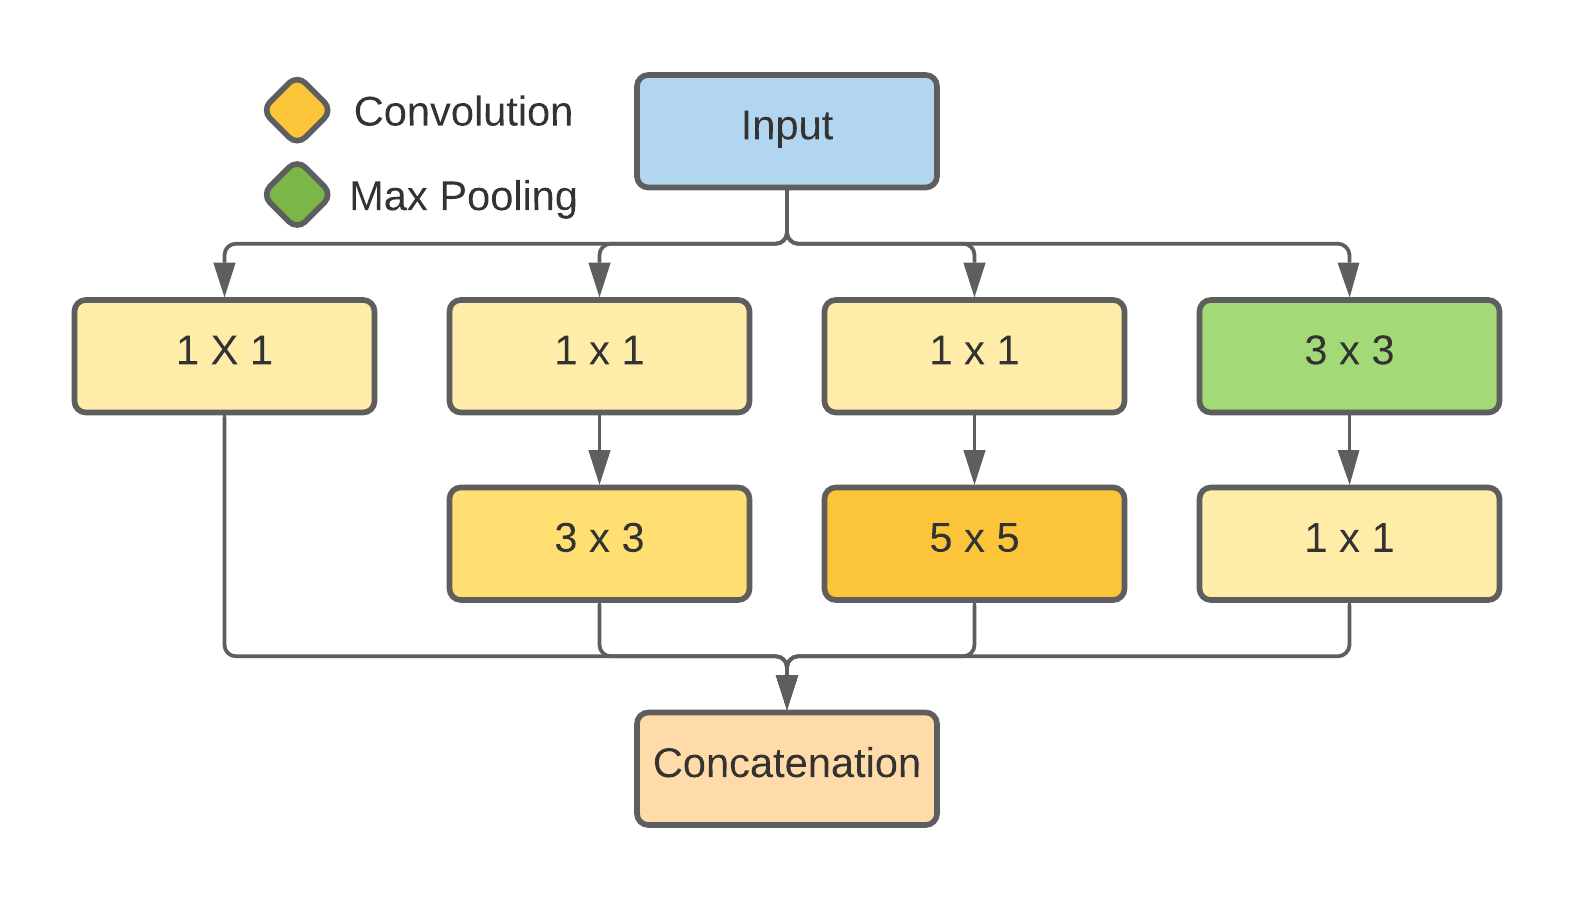
\includegraphics[width=0.5\textwidth]{InceptionModule}
    \caption{\label{fig:InceptionModule}Inception Module Example.}
  \end{wrapfigure}
  On of the first major pioneering works in the field of machine vision has been \cite{Cun1989} which designed a CNN architecture to be used for character recognition and printed on a chip. With all of it's 49 templates (today known as filters) being designed by hand. And later goes on to to introduce 'Digit Recognition Using Constrained Automatic Learning' which allows some parameters of the network, including filter values to be updated automatically via backpropogation, removing the problem of having to design all of the filters manually. Manually designing filters can be seen as introducing some priori information to the network. Which also aleviates the problem of having a scarce amount of data. A noteworthy step when training their network is the final stages of training whereby they waited for their model to converge at a minima (minimizing loss, i.e. error) which took 23 learning passes, then trained it for a further 5 passes on a dataset that quote "had undergone slightly different preprocessing", resulting finally in a 5\% error rate at classifying handwritten digits. Later in the work of creating LeNet5 \cite{LeCun1998} we see the invention of fully automated parameter tuning via backpropogation (for more on backpropogation see \cite{CunYannle1988}) that led to, acheiving 0.8\% error rate at identifying hand written digits. This was in part made possible by the increased amount of data available to train the network.
  \par
  Following from LeCun we see the next popular architecture that is often used as a benchmark in later papers AlexNet\cite{Krizhevsky}. A noteworthy aspect of it's design is the choice to change from using the tanh activation function that we find in \cite{leCun1998} to the relu activation function, which has been adopted in all state of the art aproaches today. The relu funciton is linear so we see a decrease in training time by virtue of using a function that is less computationally expensive. They found that due due to the large number of paramters in the network, it had a tendency to overfit the training set. To mitigate this, data augmentation is used including reflections and zooming in on only parts of the image such as corners/middle. This network also employs dropout as discussed later. When training the model stochastic gradient descent is used, whereby the parameters of the network are updated based on the loss of each training example. We also see mention of the concept of 'fine tuning' a network, whereby one takes a network that is pre-trained on a generalized dataset and then further trains it on domain or dataset specific input. Furthermore, we see evidence for the virtue of using ensembles of CNN's to reduce classification error. Finally the paper concludes stressing the importance of depth for classification accuracy citing a 2\% reduction in classification accuracy for top-1 performance if any convolutional layers are removed. However a later paper \cite{Zagoruyko} has established that 'widening' networks can be just as or more effective than deepening. The concept of widening can also be used to explain the effectiveness of InceptionNets.
  % We also see the idea of specialising
  \par
  The feature that sets InceptionNet architectures apart from previous iterations of CNN is the different varieties of Inception Module. An inception module is multiple convoulutional operations occuring in parallel and finally being concatenated together. Aditionally 1x1 convolutions are employed to reduce the input volume to later convolutions and therefore improve training time. This aproach is commonly refered to as 'widening' the network.
  \par
  As it stands, there are few, (if any) papers exploring the efficacy of the novel fractalNet architecture \cite{Larsson2016} for crop disease detection or on any other dataset aside from the commonly used CIFAR10 \& 100.
  \par
    \begin{wrapfigure}{R}{0.5\textwidth}
      \centering
      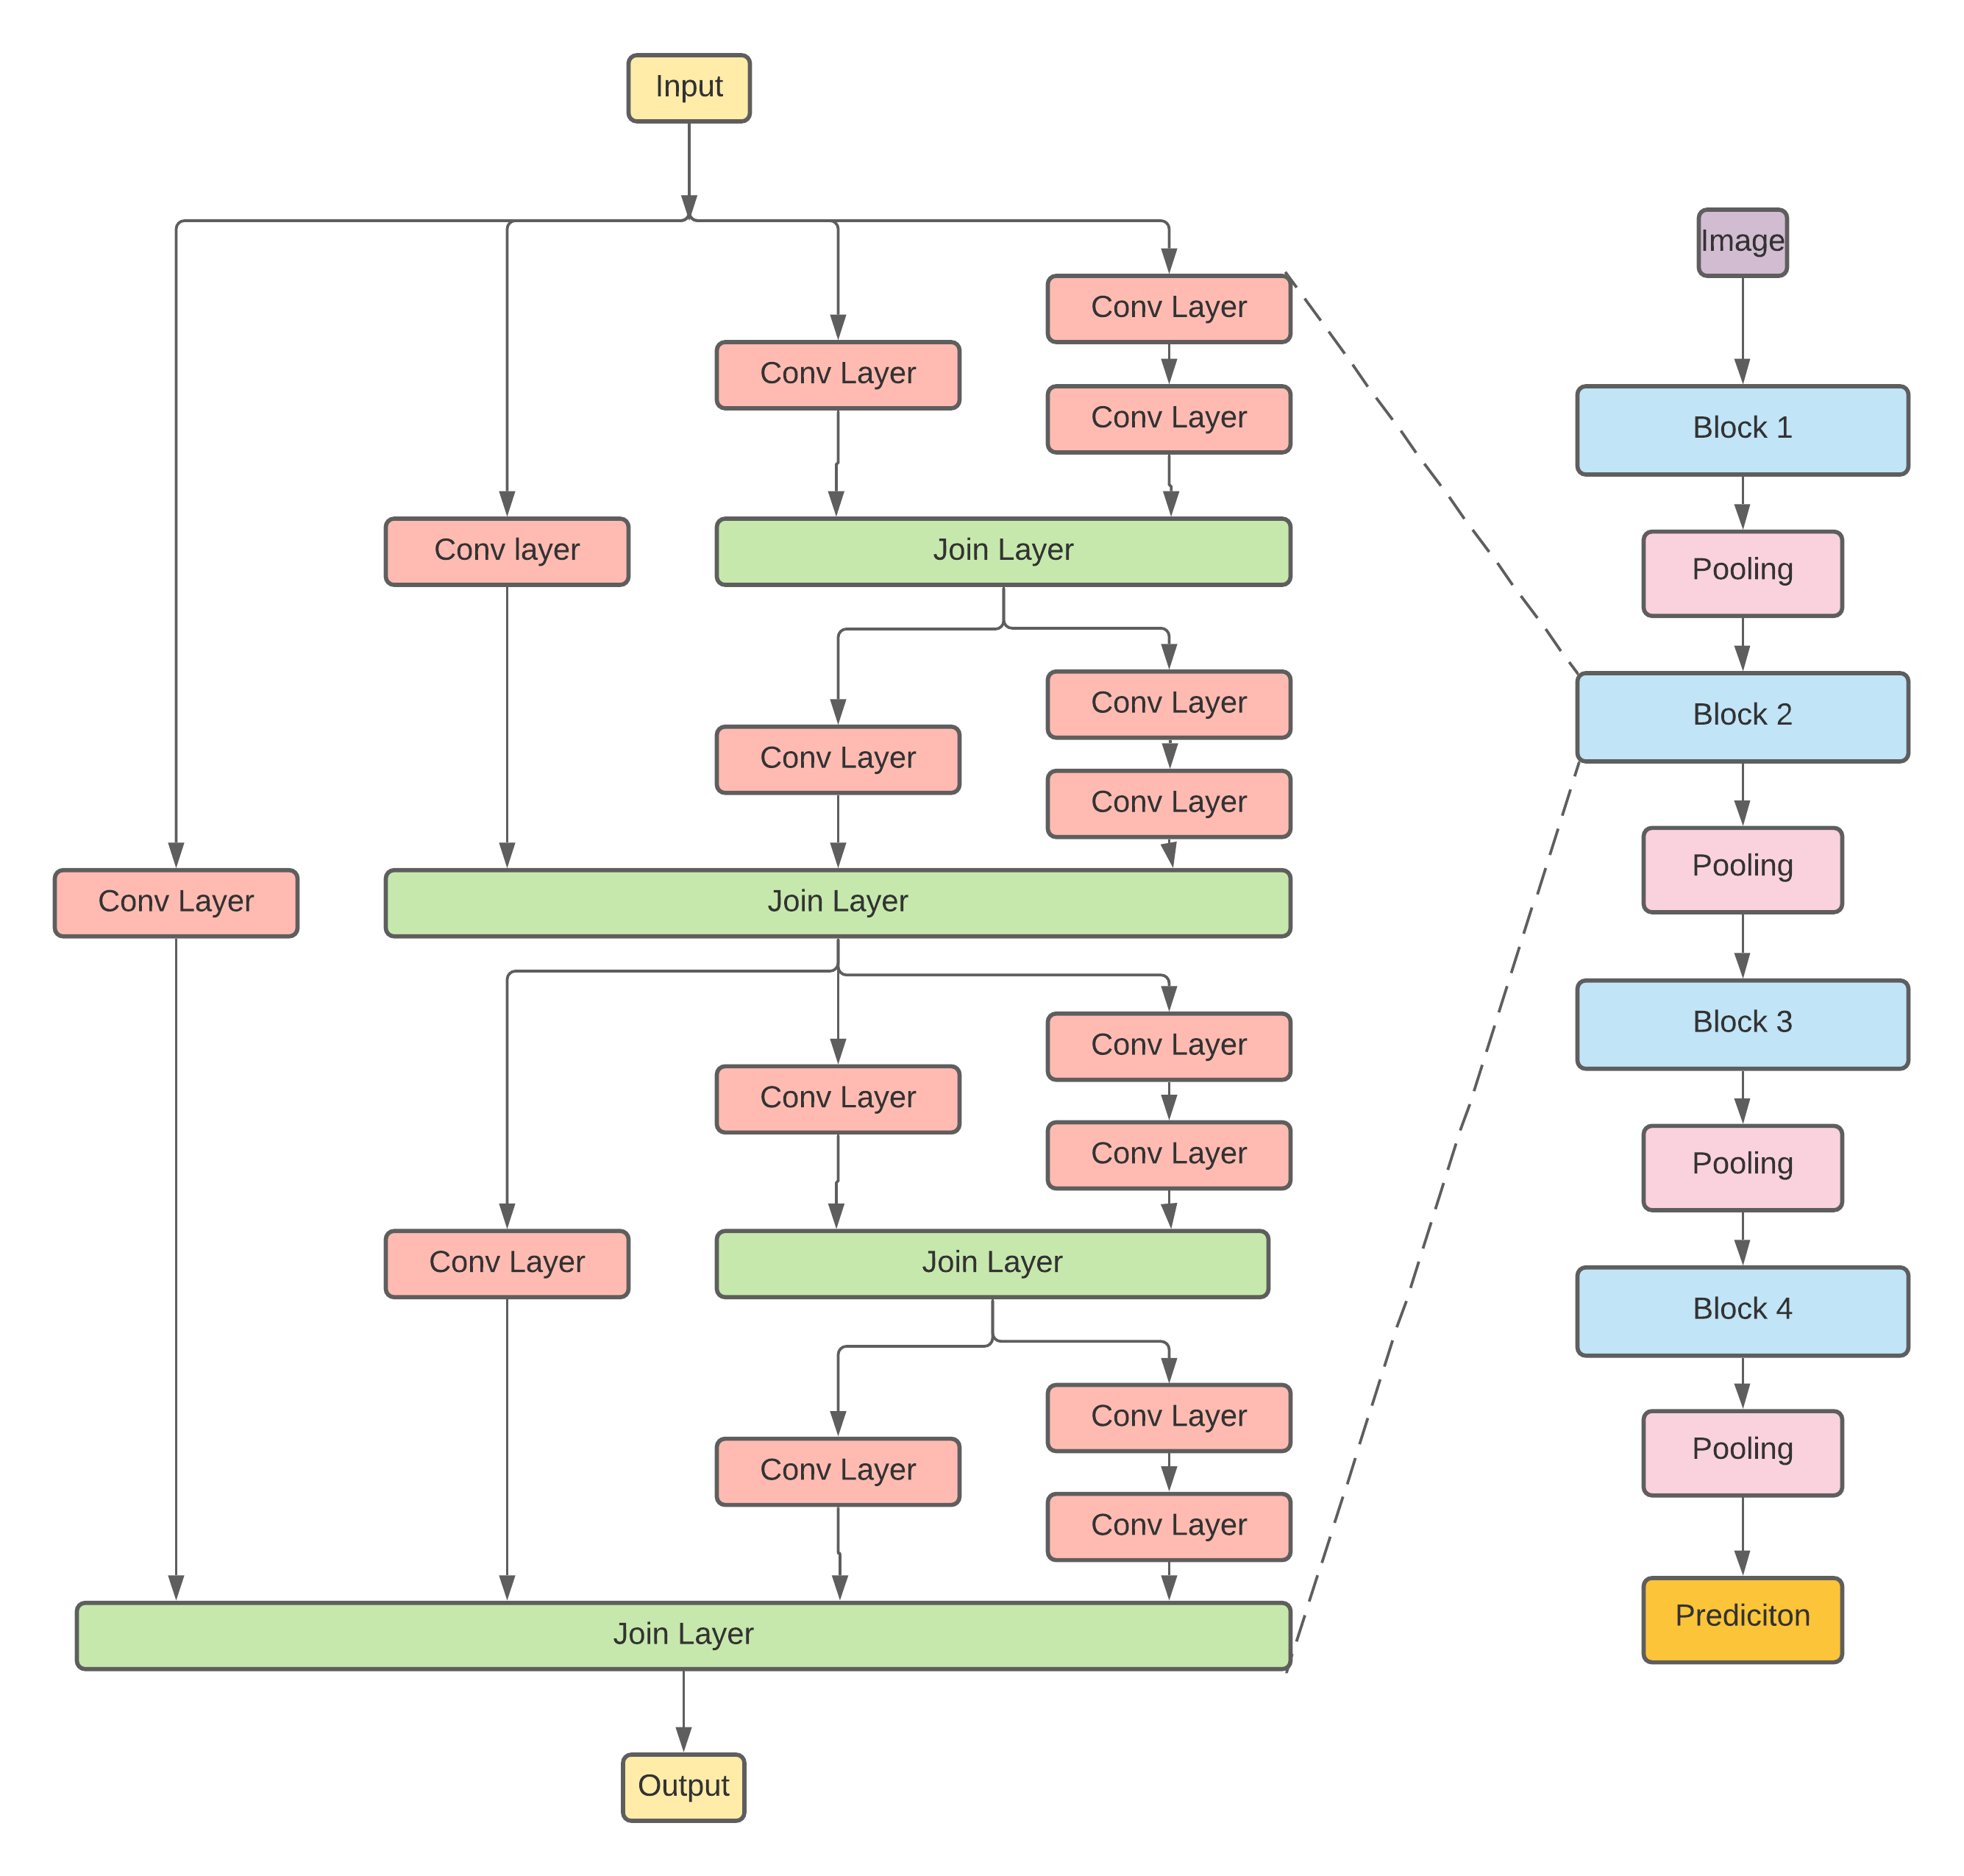
\includegraphics[width=0.5\textwidth]{Images/FractalNetArchitectureCopy}
      \caption{\label{fig:FractalNet_arcitecture}FractalNet Architecture.}
    \end{wrapfigure}
  \par
  The Inventors of the fractalNet performed experiments that justified their use over ResNets. Demonstrating results that showed improved classification accuracy. Another feature of the fractalNet architecture is the ability for the user to choose between speed of prediction and accuracy of prediciton as it is possible to take longer or shorter paths through the network. Longer paths being more accurate and more time consuming.
  \par
  Research has been conducted in 2016 \cite{Zagoruyko} that determined 'wider' networks perform better than their deep narrow counterparts. They found that their 16-layer deep network had the same accuracy as a 1000 layer thin deep network with a comparable number of parameters. With the wider network being faster to train.
  \par
  A key feature of CNN design is size and number of filters. In all examples mentioned (Resnet, InceptionNet, AlexNet etc), filter size is always odd and square. For instance 1x1, 3x3, 5x5 and so on. Size of filter will determine the size of the feature the filter will encode for. Number of filters will determine the depth of the convolution output. It is noteworthy that the Resnet50 architecture \cite{He} uses almost entirely 3x3 size filters. Whereas, the Inception module employs a mixture of 1x1 through to 5x5 convoutions.
  \par
  A technique known as dropout is a feature that has been employed in increasingly deep networks to prevent overfitting and was first introduced by \cite{Srivastava2014}. The principle behind its operation is randomly dropping paths between neurons during training. This ensures that predictions do not become overly reliant on a single (or gorup of) neuronal activation(s), that can correlate to some bias in the training data. And prevents neurons from becoming co-adaptive. This teqnique was employed in AlexNet \cite{Krizhevsky} whereby they used dropout in the first two fully connected layers of their model. They found that using dropout prevented overfitting but made training take twice as long. This exact method whereby dropout is used in the first two fully-connected layers is seen again in VGGNet\cite{Simonyan2015} which performed experiments on several different architectures, concluding the efficacy of deepening networks to acheive higher classification accuracy. Both methods choosing to employ a dropout chance of 50\%.
  \par
  Another aspect of CNN's is the process by which they progressively narrow down the possibilities until they arrive at their conclusion. This is done by encoding loose abstract forms that relate to groupings of objects in the early layers and gradually arriving at very generalized forms such as horizontal lines or sine waves in the later layers. So to give an example drawn from the AI microscope [CITE AI MICROSCOPE] . In an early layer  we may find a neuron that encodes for two seemingly unrelated objects such as dogs and turnstiles, a middle layer may encode for things under the sea or star shaped objects. Final layers encode for more generic features such as diagonal lines or squares. %In the case of the dog and the turnstile, one can observe that a 'branch' of a turnstile is equateable to the leg of a dog and the 'console?' of the turnstile be equateable to the dogs body.
  \par

  \begin{landscape}
    \begin{figure}[H]
      \begin{center}
        \includegraphics[scale=0.7]{Images/InceptionLayers/LayerExamples}
        \caption{InceptionNet Filter Activation Maps}
        \label{fig:inceptionNet_filter_activation}
      \end{center}
    \end{figure}
  \end{landscape}
  \par

  \newpage


\section{Problem Definition}
  As it stands there are currently (09/02/2021) no easily found \footnote[1]{(i.e. not present in the first 3 pages of a google search for 'crop defect identification' and 'What's wrong with my crop')} web interfaces for interacting with a crop defect identification service.
  \par
  Although there exists very capable publicly available image classification networks. \cite{Yandex} There is no bespoke application catering soley to crop defect identification, that has the benefit of providing recourse information to the user.

\section{Proposed Solution}
  To provide a web service that interacts with a convolutional neural network (CNN) backend to diagnose crop defects such as, nurturing problems e.g. lack of water/nitrogen/C02, too hot/cold. And external threats such as crop disease/pest infestation. The interface will be simple and intuitive as possible. The UI should minimise points of interaction and streamline the process of uploading a crop image to be analysed.
	The web service will return information regarding the percentage likelihood of each kind of crop defect, including images that are of similar nature to the one analysed.

\section{Aims and Objectives}
  These should be SMART with clear success criteria defined
  specific, measurable, achievable, realistic, Timebound
  \subsection{Aims}
    \begin{itemize}
      \item To aid gardneners and smallholders in identifying crop defects.
      \item To aid gardeners and smallholders in taking relevant recourse.
    \end{itemize}
  \subsection{Objectives}
    \begin{itemize}
      \item Provide a way for a user to upload an image to be analysed.
      \item Display infomration regarding the likelihood of each kind of defect.
      \item Display recourse information alongside defect information.
      \item Have gallery of images filtered by crop and disease type.
    \end{itemize}

\section{Risk Table}
  % \begin{center}
  % \begin{tabular}{c c c c c}
  %   \hline
  %   ID & Name & Likelihood & Impact & Control Mechanisms \\ [0.5ex]
  %   \hline\hline
  %   01 & Improper Time Management & Med/Low & High & Staying On-track to the Gantt Chart \\
  %   02 & HDD/Storage failure & Low & High & All work will be backed up to github. And intermitently to Google Drive \\
  % \end{tabular}
  % \end{center}


  % Table generated by Excel2LaTeX from sheet 'Risks_Table'
\begin{landscape}
  \begin{table}[ht]
    \centering
    \caption{Risks Table}
      \begin{tabular}{| c | c | c | c | c |}
      \toprule
      ID & Name & Likelihood & Impact & Control Mechanisms \\
      \midrule
      1     & Improper Time Management & med/low & high  & \multicolumn{1}{l|}{Follow the Gannt chart} \\
      \midrule
      2     & HDD/storage failure & low   & high  & All work will be backed\newline{} up to github \\
      \midrule
      3     & Illness/Injury & med   & med   & Should the need arise I\newline{}will apply for an extention\newline{}to the due date. \\
      \midrule
      4     & RSI (repetetive strain injury) & med   & low   & Work with proper posture\newline{}and set up workstation properly.\newline{}And take frequent breaks \\
      \midrule
      5     & Eye strain & med   & low   & Ensure room is well lit when working\newline{}on a screen.  \\
      \midrule
      6     & Incorrect Task Prioritisation & med   & med   & Iteratively re-asses the work being\newline{}done and compare it to the mark\newline{}scheme. \\
      \midrule
      7     & Postural problems & med   & low   & Work with proper posture\newline{}and set up workstation properly.\newline{}And take frequent breaks \\
      \bottomrule
      \end{tabular}%
    \label{tab:risksTable}%
  \end{table}%
\end{landscape}

  (ID, name, likelihood, impact, control mechanisms / accept)

\section{Overview}
  Introducing rest of dissertation (with cross references to sections)
